\pdfoutput=1
% In particular, the hyperref package requires pdfLaTeX in order to break URLs across lines.

\documentclass[11pt]{article}

% Remove the "review" option to generate the final version.
%\usepackage[review]{ACL2023}
\usepackage{ACL2023}

% Standard package includes
\usepackage{times}
\usepackage{latexsym}

% For proper rendering and hyphenation of words containing Latin characters (including in bib files)
\usepackage[T1]{fontenc}
% For Vietnamese characters
% \usepackage[T5]{fontenc}
% See https://www.latex-project.org/help/documentation/encguide.pdf for other character sets

% This assumes your files are encoded as UTF8
\usepackage[utf8]{inputenc}
\usepackage{float}
% This is not strictly necessary, and may be commented out.
% However, it will improve the layout of the manuscript,
% and will typically save some space.
\usepackage{microtype}

% This is also not strictly necessary, and may be commented out.
% However, it will improve the aesthetics of text in
% the typewriter font.
\usepackage{inconsolata}

\usepackage{graphicx}

% If the title and author information does not fit in the area allocated, uncomment the following
%
%\setlength\titlebox{<dim>}
%
% and set <dim> to something 5cm or larger.

\title{Probing Small Vision-Language
Models for Global and Local Semantic
Representations}

% Author information can be set in various styles:
% For several authors from the same institution:
% \author{Author 1 \and ... \and Author n \\
%         Address line \\ ... \\ Address line}
% if the names do not fit well on one line use
%         Author 1 \\ {\bf Author 2} \\ ... \\ {\bf Author n} \\
% For authors from different institutions:
% \author{Author 1 \\ Address line \\  ... \\ Address line
%         \And  ... \And
%         Author n \\ Address line \\ ... \\ Address line}
% To start a seperate ``row'' of authors use \AND, as in
% \author{Author 1 \\ Address line \\  ... \\ Address line
%         \AND
%         Author 2 \\ Address line \\ ... \\ Address line \And
%         Author 3 \\ Address line \\ ... \\ Address line}

\author{Jonathan Schwab \\
  {\small\texttt{jonathan.schwab@student.uni-tuebingen.de}} \\\And
  Tsun Wai Wong \\
  {\small\texttt{tsun-wai.wong@student.uni-tuebingen.de}} \\}

\begin{document}
\maketitle
\begin{abstract}

\end{abstract}


\section{Introduction}
Vision--language models (VLMs) combine text and image understanding and have become central to multimodal AI research. Probing studies help to uncover how such models encode semantic information at different layers, complementing evaluations on end tasks. A recent study \cite{tao2024probingmultimodallargelanguage} examined decoder-only multimodal models such as Kosmos and LaVIT, and found that global semantics are most strongly represented in intermediate layers, while upper layers shift toward local, token-level information, which can reduce the ability to encode global meaning.
In this work, we extend this line of analysis to recently released compact models such as Qwen2-VL-2B and FastVLM-0.5B. These models represent a new generation of efficient VLMs with parameter counts in the low billions, designed for practical deployment under limited resources. Whether their internal representational patterns follow the same global–local layering observed in earlier models, or show different dynamics, remains an open question.
To address this, we developed a general probing framework that enables layerwise representation extraction, flexible pooling of token embeddings, and efficient training of lightweight classifiers. Using this framework, we construct two probing tasks on MS~COCO \cite{lin2014microsoft}: a caption–image entailment experiment probing global semantics, and an object-category experiment probing local semantics. Following established methodology \cite{alain2018understanding}, we freeze the VLM parameters, pool hidden states into fixed-size embeddings, and train classifiers on top. We report accuracy, precision, recall, and F1 scores per layer to quantify representational quality.
Our experiments provide insight into how current compact VLMs encode global and local information across layers, and allow comparison with trends previously reported for older models \cite{tao2024probingmultimodallargelanguage}.

\section{Methods}

\subsection{Models}
We developed a probing framework for three compact vision--language models:
\textbf{Qwen2-VL-2B} \cite{qwen2vl2024} and \textbf{FastVLM-0.5B} \cite{fastvlm2025}.
All models were used in frozen form, i.e., without updating their parameters,
so that only lightweight probing classifiers were trained on top of their internal
representations. This allows us to isolate the representational capacity of the models
at different layers without confounding effects from fine-tuning.

\subsection{Probing Tasks}
To investigate the distinction between global and local semantic representations,
we designed two probing tasks. The \emph{caption experiment} targets global features
by testing whether the model can align an image with a candidate caption.
For this task, inputs are constructed using the prompt
\begin{quote}
\texttt{This image contains: \{caption\}. Is this right?}
\end{quote}
and the probe performs binary classification of whether the caption correctly describes the image. Due to limited computational resources, we just use one positve and one negative caption per image in contrast to \cite{tao2024probingmultimodallargelanguage}.
We consider a set of images $M$ with associated ground-truth captions $C$
and a set of randomly sampled negative captions $C'$.
For each image $m \in M$, we select one positive caption $c^+(m) \in C$
and one negative caption $c^-(m) \in C'$.
This yields the dataset
\[
D = \{(m, c^+(m)), (m, c^-(m)) \;\mid\; m \in M\}.
\]
The probing classifier is then trained to solve the binary decision problem
\[
f : D \;\rightarrow\; \{0,1\},
\]
with $f(m, c^+(m)) = 1$ and $f(m, c^-(m)) = 0$.
The \emph{category experiment} focuses on local features by probing whether the model
can identify the presence of specific objects. For this task, 2 different versions of prompt have been tried out in the experiment.
Initially, the prompt take the form
\begin{quote}
\texttt{This image contains the following types of object: \{categories\}}
\end{quote}
After reviewing the preliminary results, a prompt without the list of the object categories is implemented to prevent data leakage.
\begin{quote}
\texttt{This image contains the following types of object: }
\end{quote}
and the probe must predict the existence of each category in the image. $\mathcal{K}$ denotes the set of object categories, and for each image $m \in M$,
the subset $K(m) \subseteq \mathcal{K}$ specifies the categories present in $m$.
The probing task amounts to learning a classifier
\[
f : M \;\rightarrow\; \{0,1\} ^{|\mathcal{K}|},
\]
such that for an image $m$, the prediction $f(m)$ is a binary vector whose positive entries correspond to the categories in $K(m)$.
Both tasks are based on the MS~COCO dataset \cite{lin2014microsoft}, which provides annotations
for images, including captions for each image. We created
training and evaluation splits. Due to limited computational resources, we restrict our analysis to a random subset of 20.000 images for the training set and 2.000 images for the evaluation set in both experiments.



\subsection{Representation Extraction}
Our framework computes hidden representations for every transformer layer of a model
given an image--prompt pair. From the token-level hidden states, we derive pooled embeddings
that serve as inputs to the probing classifiers. We implemented a general-purpose
\texttt{pool\_tokens} function that supports multiple pooling strategies, including
CLS token extraction, mean pooling across valid tokens, max pooling, token-index selection,
and a default strategy that retrieves the last non-padding token. Unless otherwise noted,
we employ mean pooling, which aggregates information across the entire input sequence
while respecting attention masks. This yields a single fixed-size vector per input
and per layer, enabling layerwise comparison of representational quality.
Moreover, our framework stores all extracted representations in a binary format,
facilitating efficient reuse and analysis without redundant computation.


\subsection{Probing Classifiers}
On top of the pooled embeddings, we train lightweight classifiers that map the
representations to task labels. For both experiments, we use a simple linear
projection with dropout regularization, optimized with Adam and cross-entropy loss.
The caption experiment is framed as binary classification, while the category experiment
is treated as multi-label prediction with label and mask vectors indicating valid
categories for each image. A set of 3 valid categories are used for the category experiment.
It typically consists of 1-2 positive categories and randomly sampled negative categories,
ensuring a balanced ratio of both. All probes are trained independently per layer, which allows
us to quantify how well each layer captures global or local semantic information.
Our trainer additionally computes detailed evaluation metrics, including accuracy for
caption entailment and macro-averaged F1, precision, recall, and confusion matrix
statistics for category recognition.

\subsection{Experimental Workflow}
In both experiments, the workflow follows the same high-level structure.
Datasets are preprocessed and split into training and evaluation sets, with
balanced numbers of positive and negative instances. The target model is then
loaded, and representations are computed for all inputs. Probing classifiers are subsequently trained
and evaluated for each layer. After finishing one model, GPU memory is released
and the next model is processed in the same way. The probing results across
layers and models are then aggregated for analysis. This setup ensures that
our experiments are efficient, reproducible, and directly comparable across
models of different architectures and scales.


\section{Results}
To evaluate the performance of the probing classifiers across different layers
and models, we generated a series of plots that visualize key metrics.
For the caption experiment, which focuses on global semantic features, the accuracy per layer
across all three models is shown in Figure~\ref{fig:accuracy_per_layer}.
Thus the positive and negative examples are balanced, a random baseline would achieve 50\% accuracy.
We can see that both probes show a similar evulution in accurancy over the most layers, with Qwen2-VL-2B performing slightly better than FastVLM-0.5B.
The accurancy increases from the first towards the later layers.
Interestingly, the accurancy of FastVLM-0.5B drops significantly in the last layers, while it remains relatively stable for Qwen2-VL-2B.

\begin{figure}[H]
    \centering
    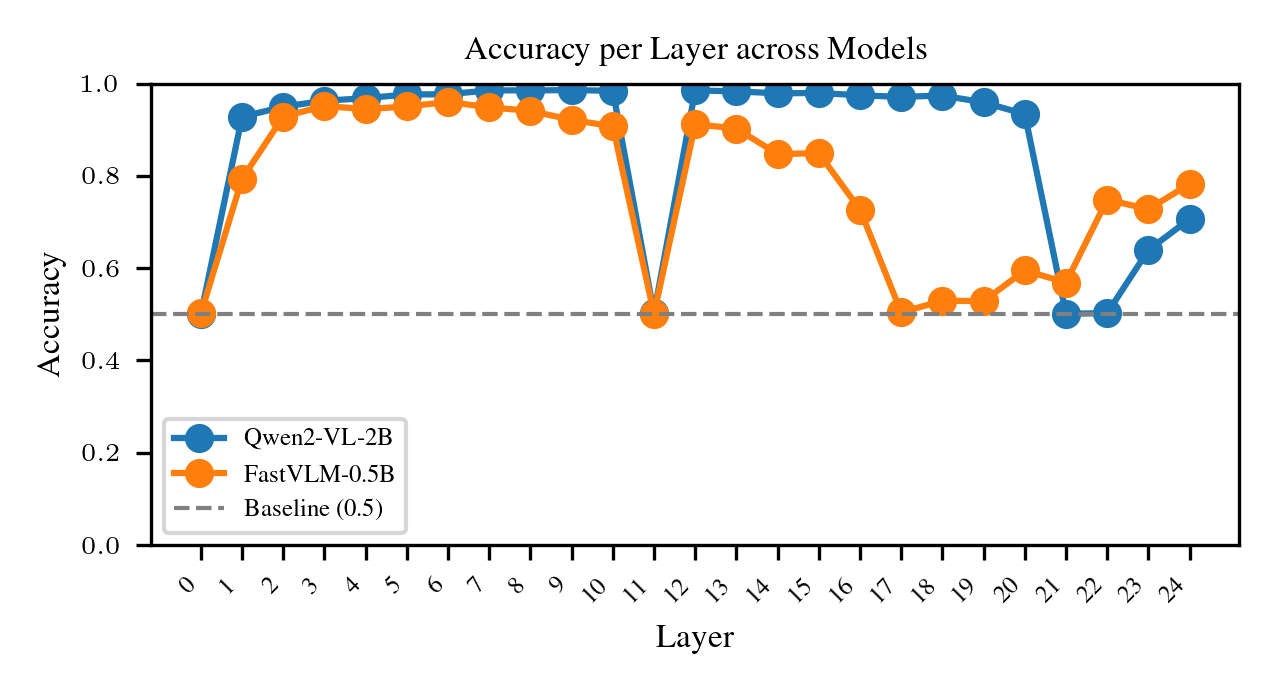
\includegraphics[width=1\linewidth]{figures/global/_combined_exp1/accuracy_lines_per_layer.png}
    \caption{Accuracy per layer across all three models.}
    \label{fig:accuracy_per_layer}
\end{figure}
In \ref{fig:combined_metrics_per_layer}, we present a heatmap that summarizes the precision, recall, and F1 scores for the caption experiment across all layers and models.
Here we can also observe a similar trend as for the accuracy. The scores are increases from the first towards the later layers and FastVLM-0.5B shows a significant drop in the last layers.
\begin{figure}[H]
    \centering
    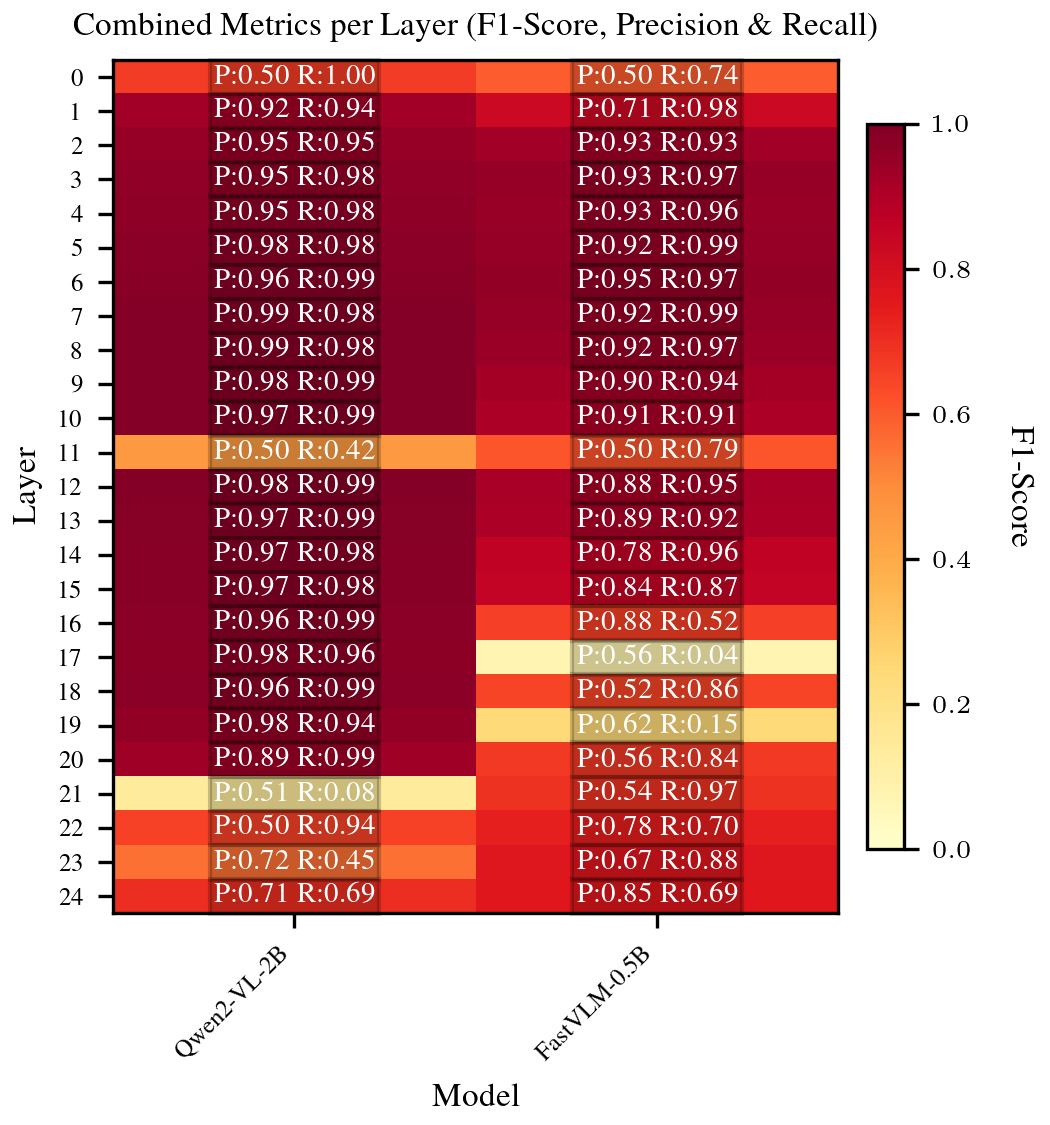
\includegraphics[width=1\linewidth]{figures/global/_combined_exp1/combined_metrics_heatmap.png}
    \caption{Precision, Recall and F1 per layer across all three models.}
    \label{fig:combined_metrics_per_layer}
\end{figure}

For the category experiment on local semantics, the accuracy per layer across the two models is shown in Figure~\ref{fig:f1_per_layer_local}.
We can see that both Qwen2-VL-2B and FastVLM-0.5B maintain a consistently high F1 scores of around 93--96\% across all layers.
In contrast to the global semantic results, here the F1 scores do not show a clear upward trend with increasing layer depth, but instead remains stable throughout.
Moreover, no significant drop is observed in the final layers for FastVLM-0.5B, with both models performing nearly identically at each layer.

\begin{figure}[H]
    \centering
    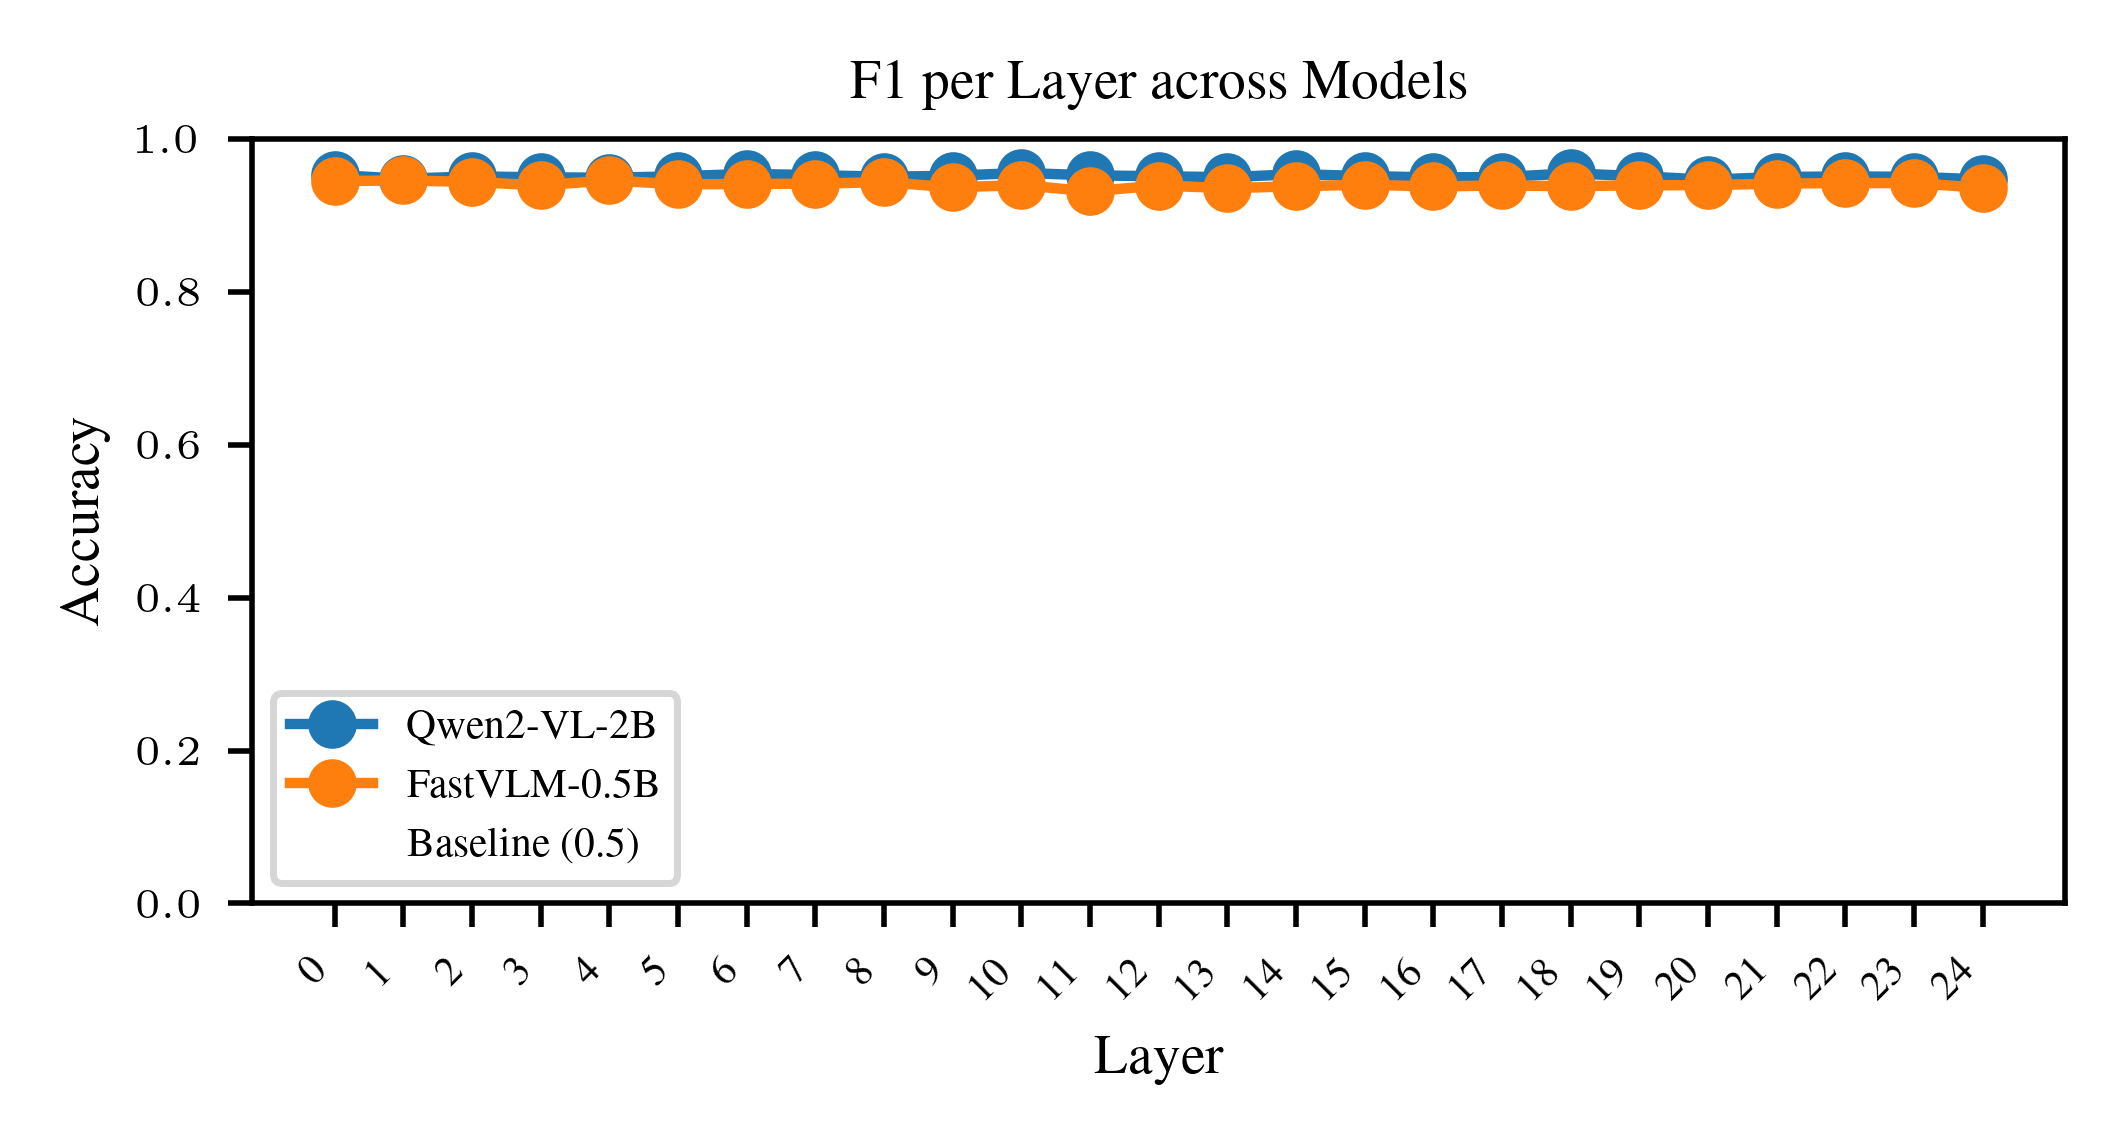
\includegraphics[width=1\linewidth]{figures/local/_combined_exp2/f1_lines_per_layer.png}
    \caption{F1 score per layer across all two models in category experiment.}
    \label{fig:f1_per_layer_local}
\end{figure}

In Figure~\ref{fig:combined_metrics_per_layer_local}, we present a heatmap that summarizes the precision, recall, and F1 scores for the category experiment across all layers and models.
These metrics confirm the same pattern as the accuracy plot: both models achieve consistently high precision and recall (around 0.94 to 0.97) across all layers, leading to stable F1 scores close to 0.95.

\begin{figure}[H]
    \centering
    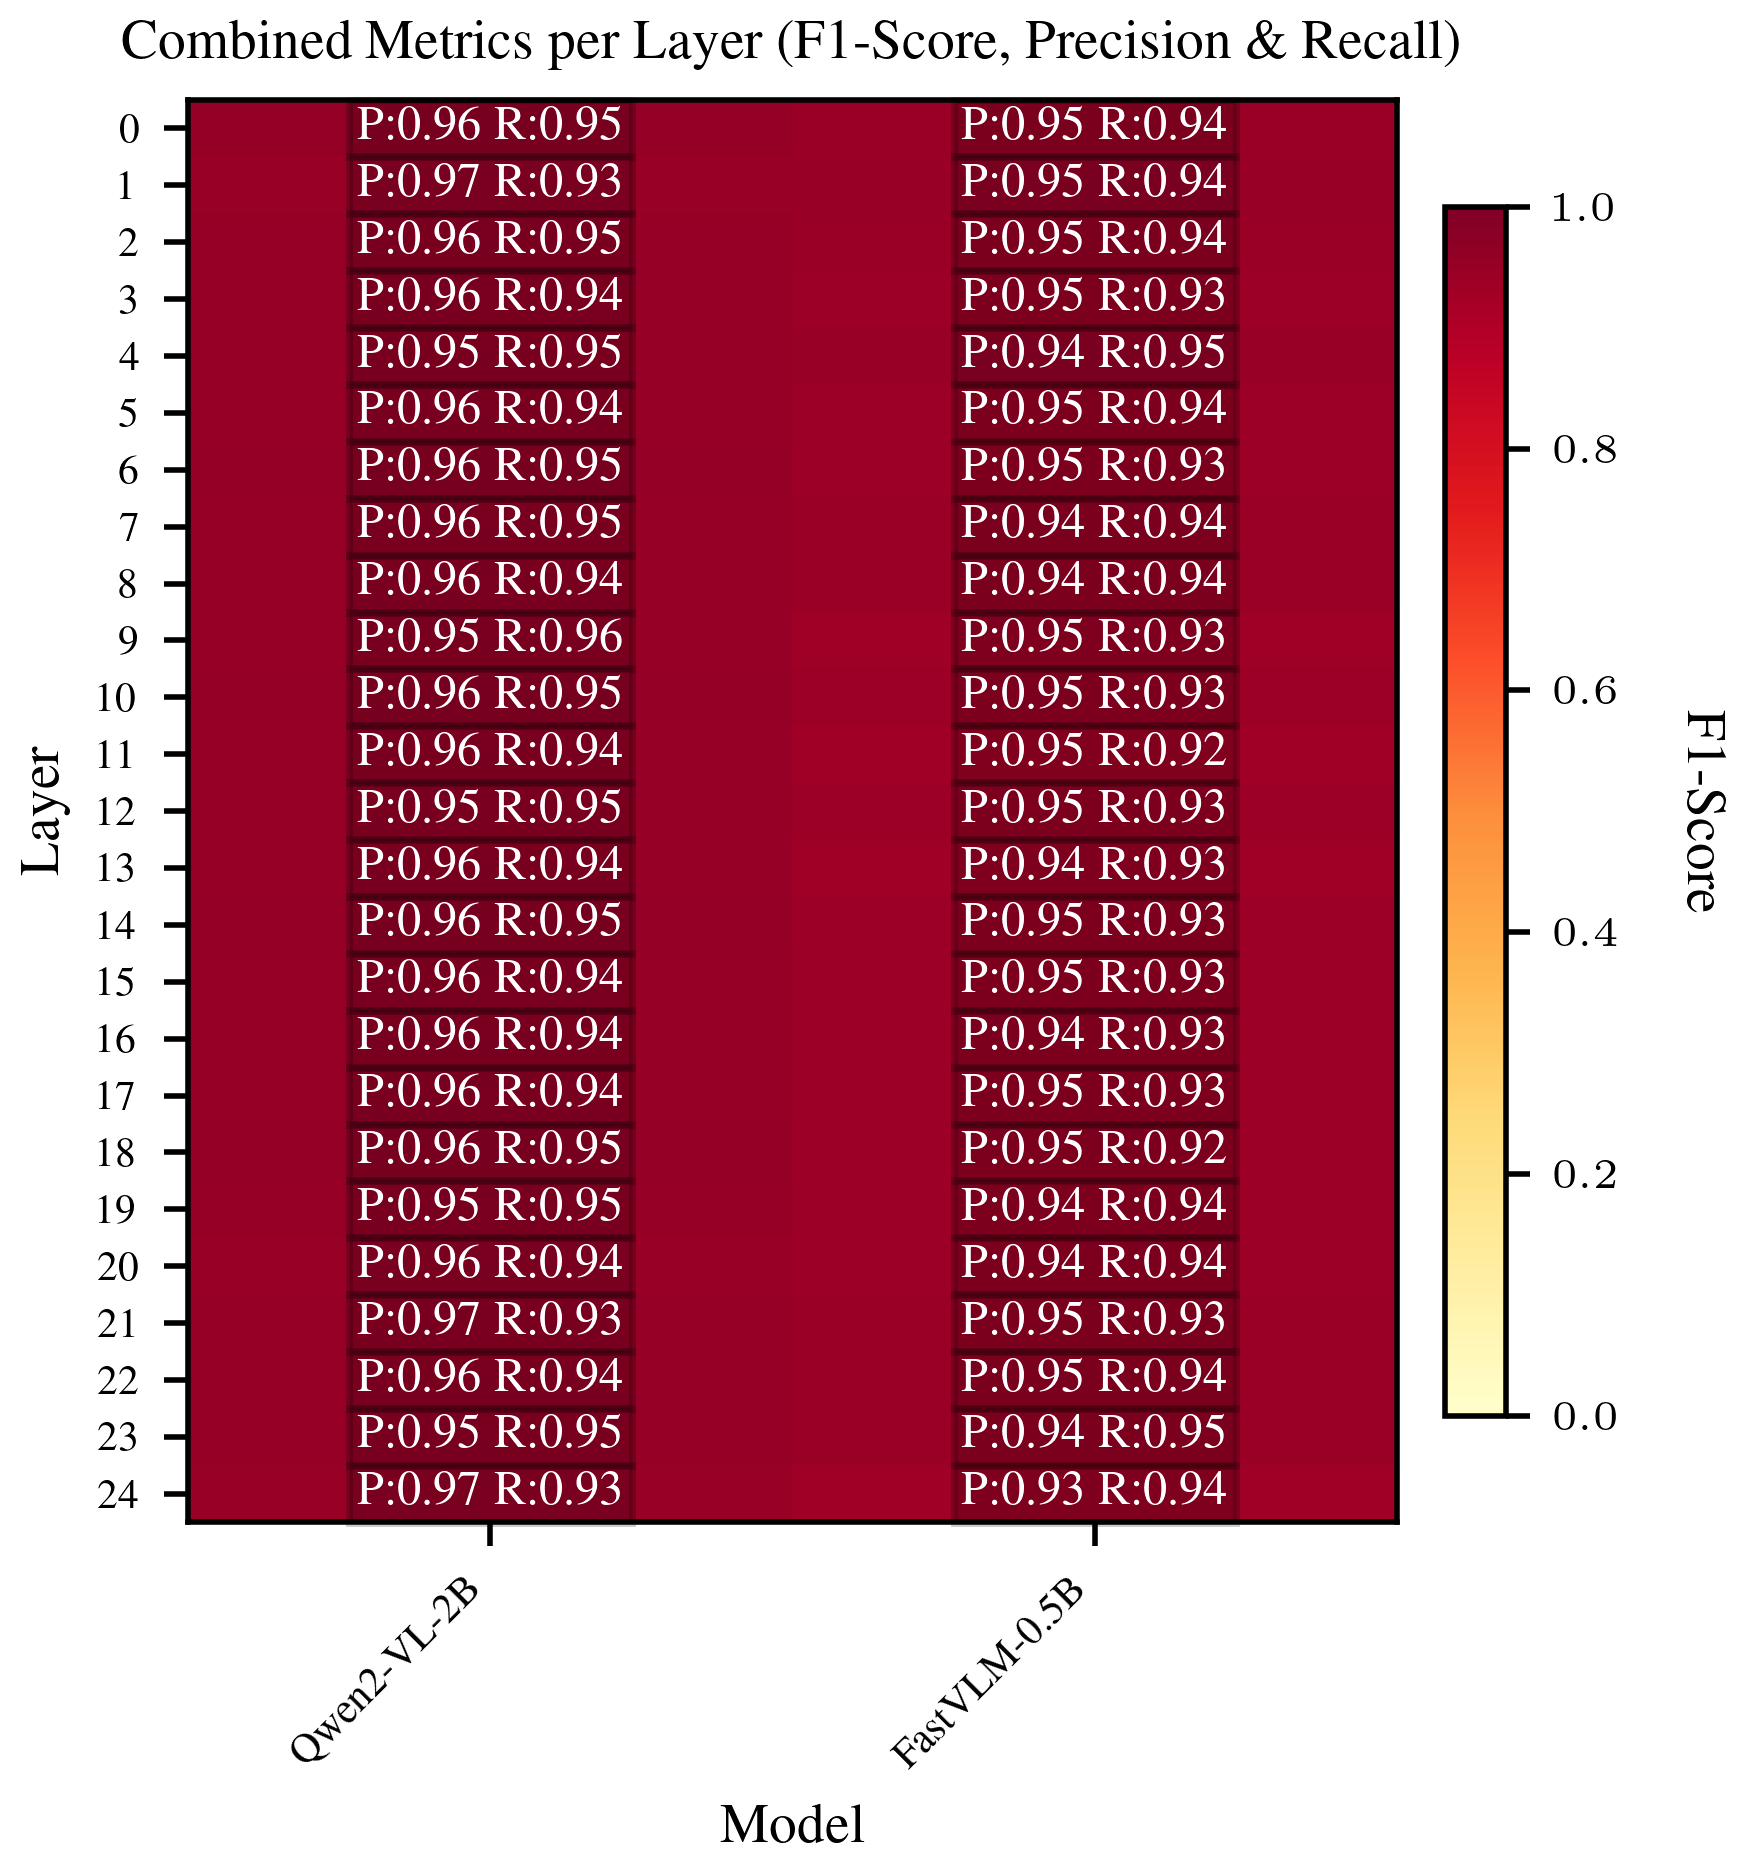
\includegraphics[width=1\linewidth]{figures/local/_combined_exp2/combined_metrics_heatmap.png}
    \caption{Precision, Recall and F1 per layer across all two models in category experiment.}
    \label{fig:combined_metrics_per_layer_local}
\end{figure}


\section{Discussion}
\subsection{Reflection on the Results}
In relation to our central research question regarding whether small VLMs follow the same global–-local representational trends observed in larger models \cite{tao2024probingmultimodallargelanguage}.
Our findings reveal both convergences and divergences.\\

In terms of global semantics, we find evidence of a consistent pattern.
In smaller models, as in larger ones, intermediate layers encode stronger global semantics than very early layers.
This is reflected in the improved performance of middle–later layers on the caption entailment probe.
In particular, both Qwen2-VL-2B and its larger counterpart Qwen2-VL-7B maintain relatively constant performance into the later layers, without an obvious decline.
However, the dynamics toward the later layers of some other models diverge.
Some larger VLMs (e.g. Kosmos-2 and LaVIT) exhibit gradual decline in global information after their peak in intermediate layers.
Meanwhile, FastVLM-0.5B shows a different behavior, with a sharp drop in performance at the final layers.\\

In terms of local semantics, our findings suggest that local semantic information is represented in a consistent manner across different layers.
Specifically, both the small-scale FastVLM-0.5B and the larger Qwen2-VL-2B encode object-level semantics in a highly linearly separable fashion throughout nearly all layers, with high F1 scores and only minor variation across depth.
Unlike larger VLMs show a clear improvement in local semantic encoding from early to mid layers. Our results show that small VLMs already capture local semantics at high fidelity from early layers.
This may suggests that smaller VLMs may be saturating their ability to encode local semantics earlier in the architecture

\subsection{Limitation of the Study}
One of the limitations of our study concerns the way negative examples were constructed. We rely on random sampling to generate negative samples of captions and categories, without accounting for their semantic closeness to the correct choice.
A previous study \cite{roesch2024EnhancingConceptualUnderstandinginMultimodal} showed that using hard negatives enables models to encode subtler distinctions, leading to stronger fine-grained conceptual understanding.
By analogy, when probing to uncover where such information is stored across layers, if the negatives are too easy, layer-specific variation may be underestimated.
This may partly explain why our local semantic probes exhibited similar performance across layers as the distinctions of the classifiers may be flattened. \\

Another limitation of our study lies in the choice of pooling strategy for sequence representations.
We applied mean pooling across valid tokens to obtain a single vector representation of the input. This approach implicitly treats all tokens as equally informative.
Prior work \cite{tang2024PoolingAndAttention} has shown that different pooling methods like taking the hidden state of the final token can yield different insights. Exploring alternative pooling strategies and comparing them systematically may provide a more nuanced view of how VLMs distribute information across layers. \\

Due to computational limits, our probing experiments were restricted to 20k training and 2k evaluation samples from MS COCO.
In addition, coverage of semantics variation would be a potential issue.
In particular, only 40 object types have been chosen for the probes in local semantics.
This reduced variation means probes might overestimate how well a model captures the information.

\subsection{Future Research Direction}
A possible extension of this work would be to broaden the probing framework beyond the current focus on local versus global semantics.
While this distinction of semantics captures one important perspective on how models encode information, it is only a partial lens through which to view their representational capacities.
Future studies could explore a wider taxonomy of knowledge types.
More fine-grained semantic representations, such as relational, compositional, and contextual understanding, as examined in recent probing approaches \cite{schiappa2023ProbingConceptualUnderstanding} can be explored.
Beyond relatively more literal and structural dimensions of meaning covered in this study, another potential direction is to investigate how VLMs handle deeper or more abstract forms of knowledge.
For example, in the perspective of combinational creativity \cite{peng2025ProbingandInducingCombinationalCreativity}, it would be insightful to investigate the models' ability to interpret novel combinations of familiar concepts. Such extensions would provide a richer picture of the models’ capabilities in generalization. \\

While our investigation has yielded useful insights using Qwen2-VL-2B-Instruct and FastVLM-0.5B, the architectural diversity in our models is still quite limited.
To more fully understand where and how information is stored or lost across vision-language models, future work should extend this probing to a broader set of VLM architectures.
For example, models under the architecture Encoder–decoder cross-modal fusion like BLIP-2 \cite{li2023BLIP2}, which integrate vision and language through deeper cross-attention layers, may preserve global and local semantic information differently.
Furthermore Mixture-of-Experts (MoE) architectures \cite{lin2024MoELLaVA}, which route information dynamically, may distribute semantic content in another way.


\section{Conclusion}

\section{References}
\bibliographystyle{acl_natbib}
\bibliography{custom}
\nocite{*}
\appendix

\section{Appendix}
\begin{figure}[H]
    \centering
    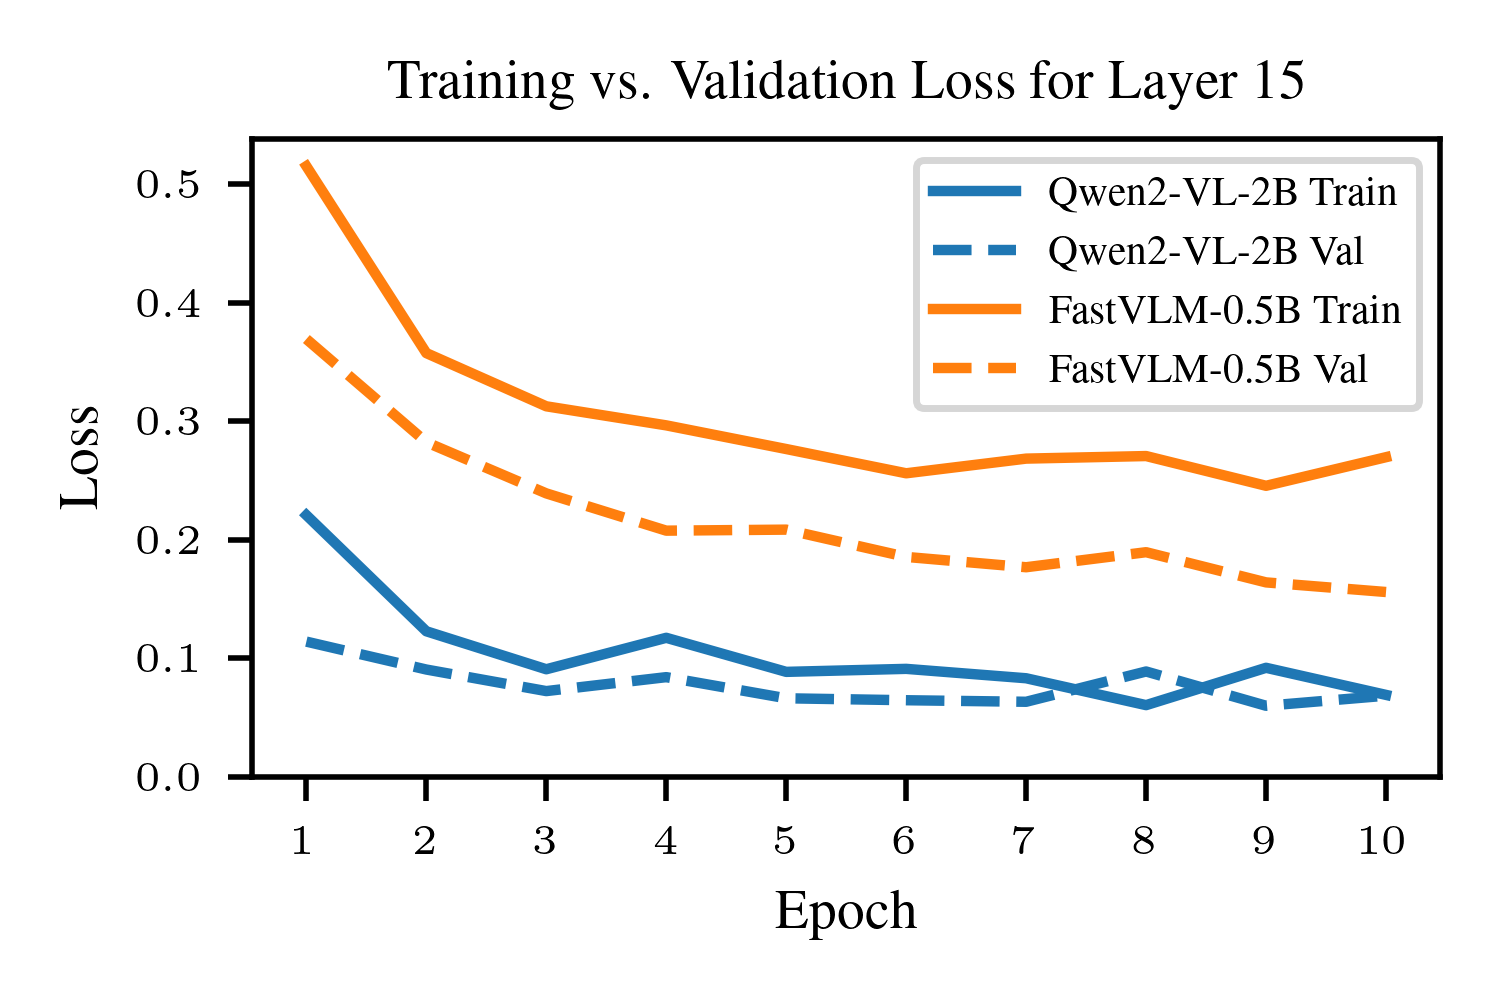
\includegraphics[width=1\linewidth]{figures/global/_combined_exp1/combined_training_progress_layer_15.png}
    \caption{A comparison of training and validation loss for the layer 15 probe (layer with best accuracy scores), analyzing model performance in the global caption experiment. The Qwen2-VL-2B model (blue) demonstrates a significantly lower and more stable loss than the FastVLM-0.5B model (orange). The small gap between the training (solid) and validation (dashed) curves for the Qwen2 model suggests robust training with no signs of overfitting. Moreover we can see that the strongest learning happens in the first 2 epochs.}
\end{figure}

\begin{figure}[H]
    \centering
    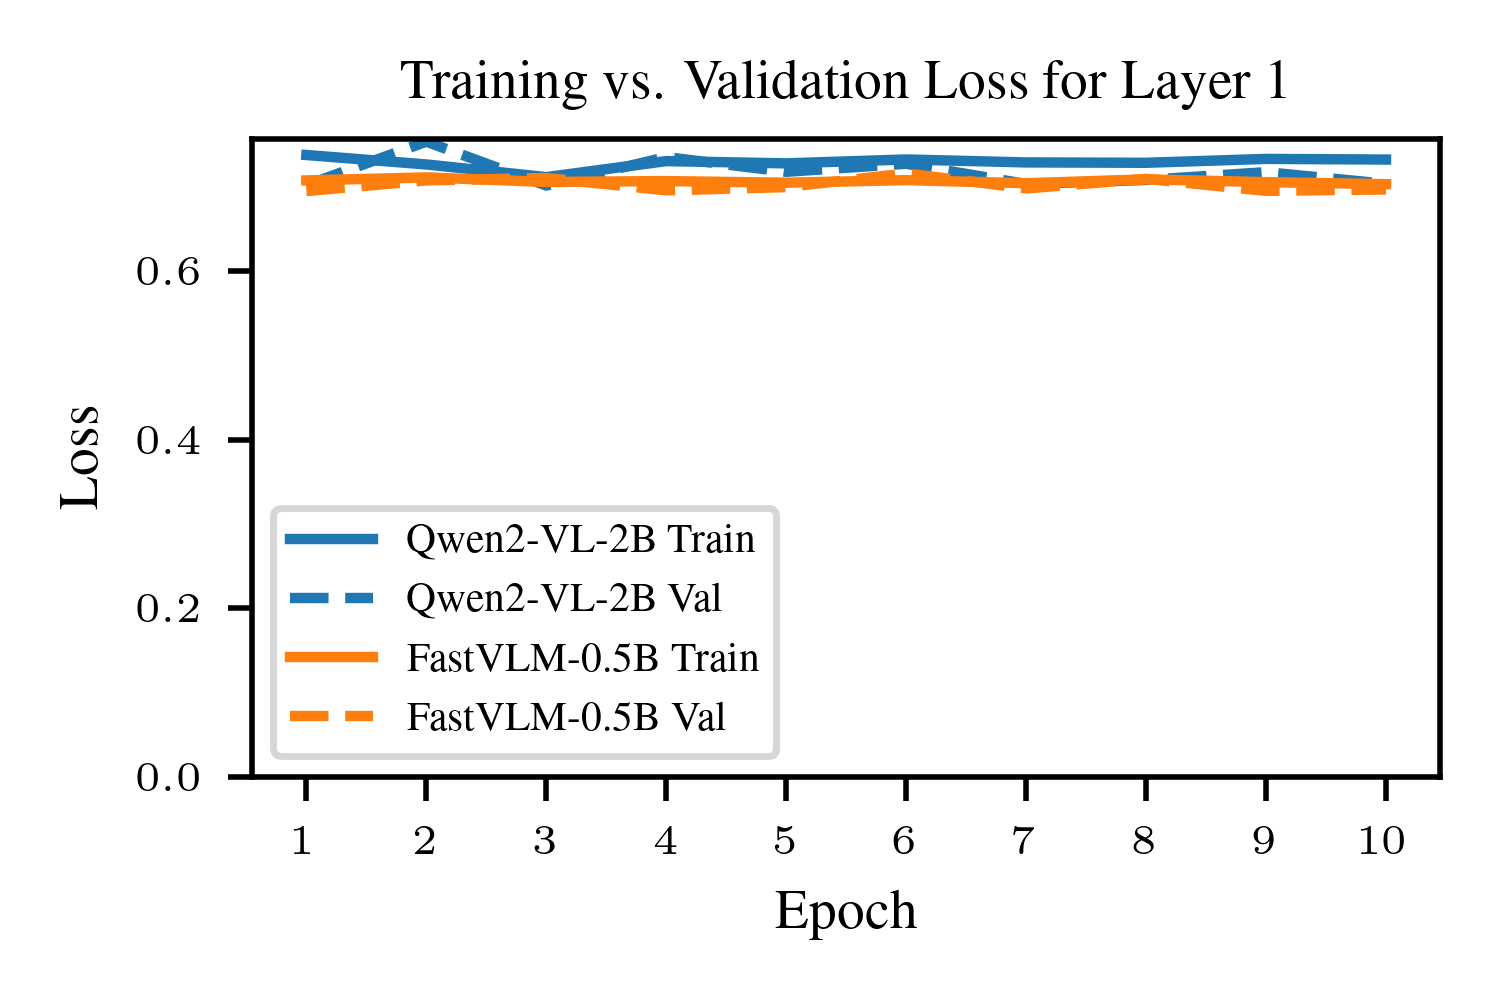
\includegraphics[width=1\linewidth]{figures/global/_combined_exp1/combined_training_progress_layer_1.png}
    \caption{A comparison of training and validation loss for the layer 1 probe (layer with lowest accuracy scores), analyzing model performance in the global caption experiment. Both models show no significant learning, with losses remaining high and stable across epochs. This indicates that the representations at this early layer do not contain sufficient information for the caption entailment task, leading to poor probe performance.}
\end{figure}

\begin{figure}[H]
    \centering
    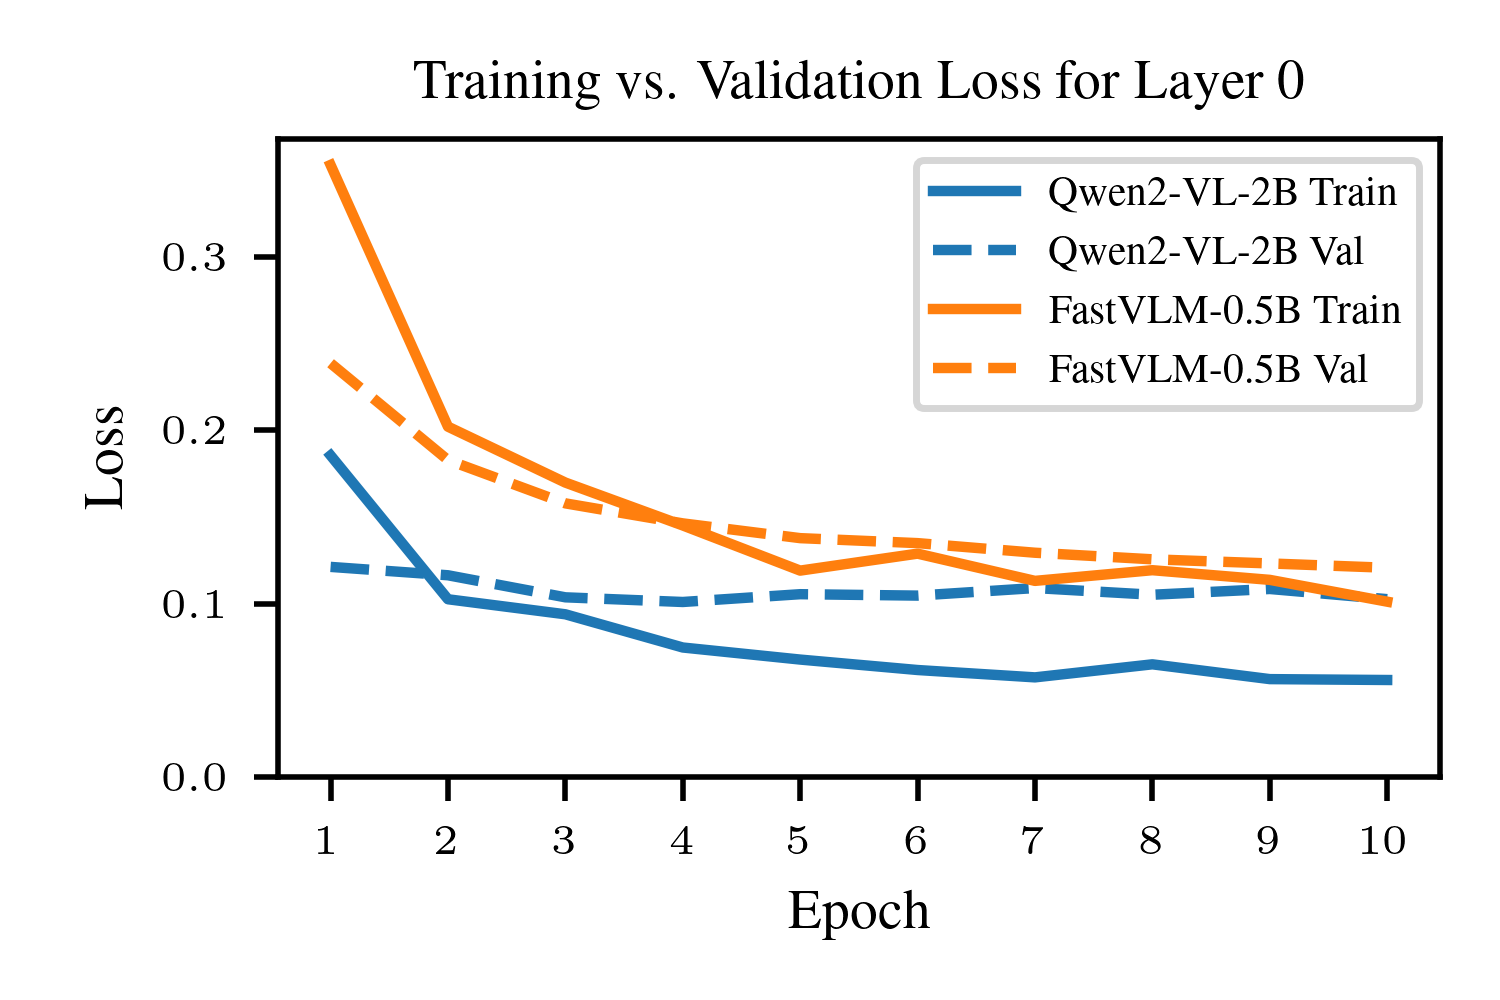
\includegraphics[width=1\linewidth]{figures/local/_combined_exp2/combined_training_progress_layer_0.png}
    \caption{A comparison of training and validation loss for the layer 0 probe (layer with best F1 scores), analyzing model performance in the local category experiment. Both models show most of their improvement within the first four to five epochs, after which the curves flatten. The Qwen2-VL-2B model (blue) achieves consistently slightly lower training and validation losses than the FastVLM-0.5B model (orange), reflecting its stronger performance overall.}
\end{figure}

\begin{figure}[H]
    \centering
    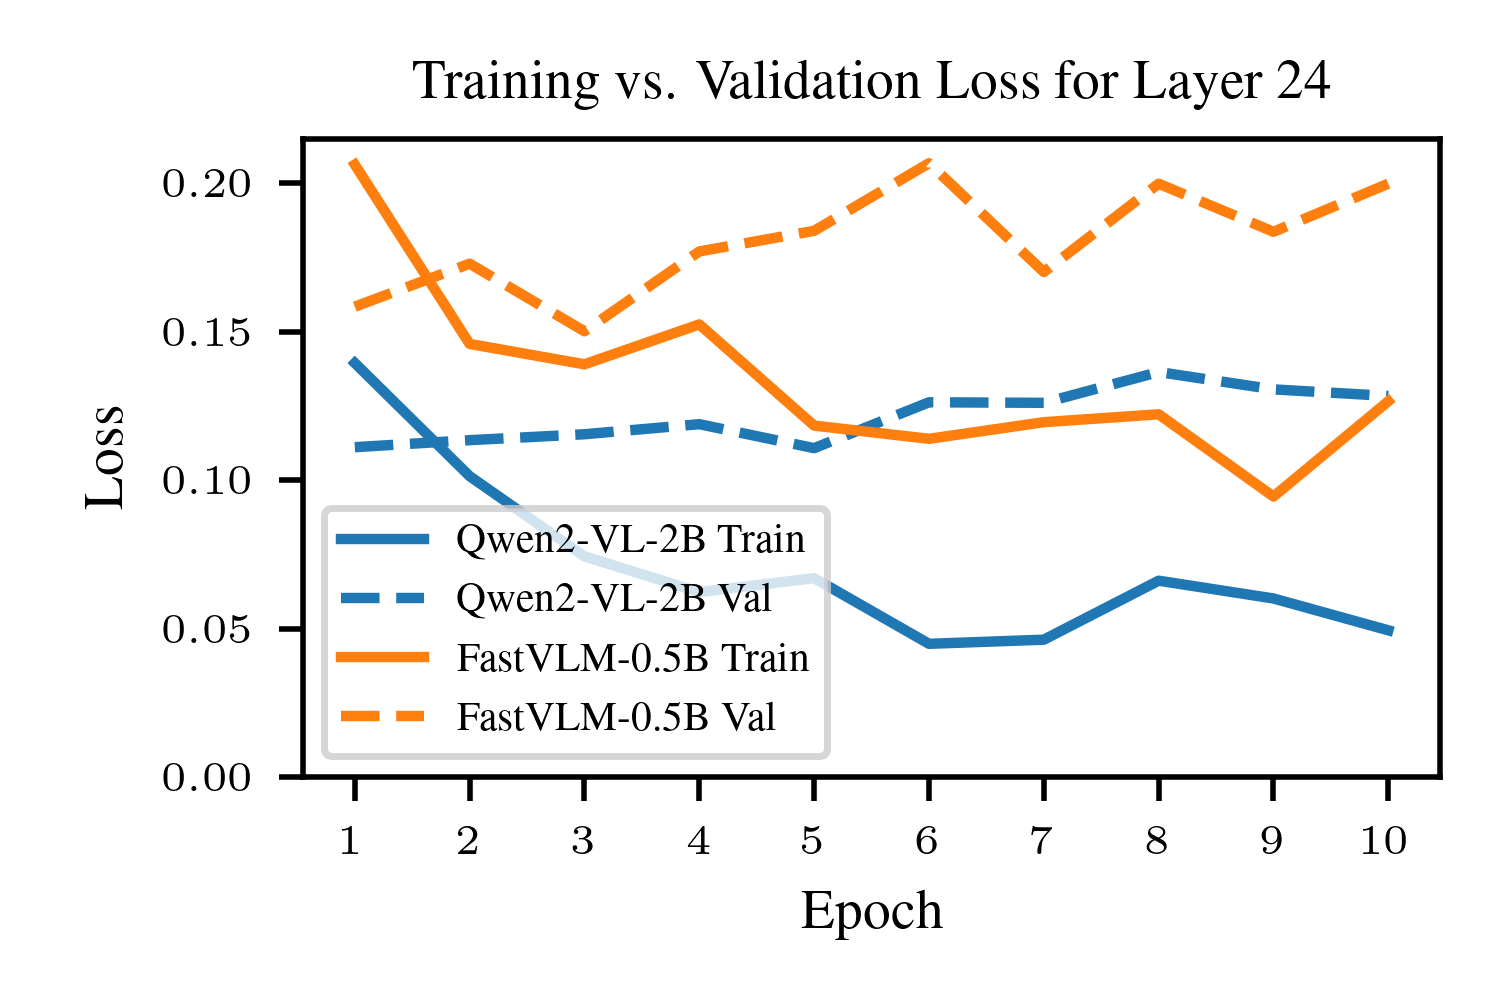
\includegraphics[width=1\linewidth]{figures/local/_combined_exp2/combined_training_progress_layer_24.png}
    \caption{A comparison of training and validation loss for the layer 24 probe (layer with lowest F1 scores), analyzing model performance in the local category experiment. Both models show limited improvement after the initial epochs, with losses remaining relatively flat overall. The validation losses remain relatively low, indicating that this layer also carries useful information for the task. The FastVLM-0.5B model (orange) shows slightly higher and less stable losses compared to Qwen2-VL-2B (blue).}
\end{figure}

\end{document}
